% ================================================================================================================
%   ____                                 _                 
%  / ___|___  _ __ ___  _ __   __ _ _ __(_)___  ___  _ __  
% | |   / _ \| '_ ` _ \| '_ \ / _` | '__| / __|/ _ \| '_ \ 
% | |__| (_) | | | | | | |_) | (_| | |  | \__ \ (_) | | | |
%  \____\___/|_| |_| |_| .__/ \__,_|_|  |_|___/\___/|_| |_|
%                      |_|                                 
% ================================================================================================================

\section{Сравнение CSG, BREP и полигональных моделей}

На~\figref{fig:DiffGeoRepr} показана одна и та же геометрическая форма, описанная в ЭВМ с помощью различных методов представления геометрии.
На панели~(а) показаны отдельные примитивы до выполнения Булевой операции. Можно видеть кривые пересечения примитивов, однако фактически уравнения этих кривых на пересечении конкретных уравнений поверхностей либо не рассчитаны вообще, либо расчитаны системой моделирования неявно исключительно для более красивой визуализации.
На панели~(b) показано твёрдое тело после выполнения Булевой операции. Здесь рёбра на пересечениях уже явно рассчитаны.
На панели~(c) показана модель после выполнения Булевой операции, триангулированная системой моделирования для визуализации, в таком режиме, когда показываются только рёбра треугольников. Отметим, что именно в такой форме, но с закрашенными треугольниками, все модели, независимо от внутреннего описания --- BREP, CSG или какое-либо другое --- визуализируются на дисплее ЭВМ. За счёт того, что угол между рёбрами треугольников, аппроксимирующими гладкое ребро исходного тела, очень мал, визуально создаётся ощущение плавных кривых.
На панели~(d) показана КЭ-модель, полученная разбиением исходной BREP модели на тетраэдральные конечные элементы с помощью пакета Netgen~\cite{NETGEN}. Видны только треугольники на поверхности, но на самом деле на тетраэдры разбито всё твёрдое тело.
Стоит отметить отличие триангуляции поверхностей для КЭ-модели и модели для визуализации. Это объясняется разными критериями алгоритма триангуляции в силу разных целей моделей.

\begin{figure}[H]
\begin{minipage}[b]{0.495\textwidth}
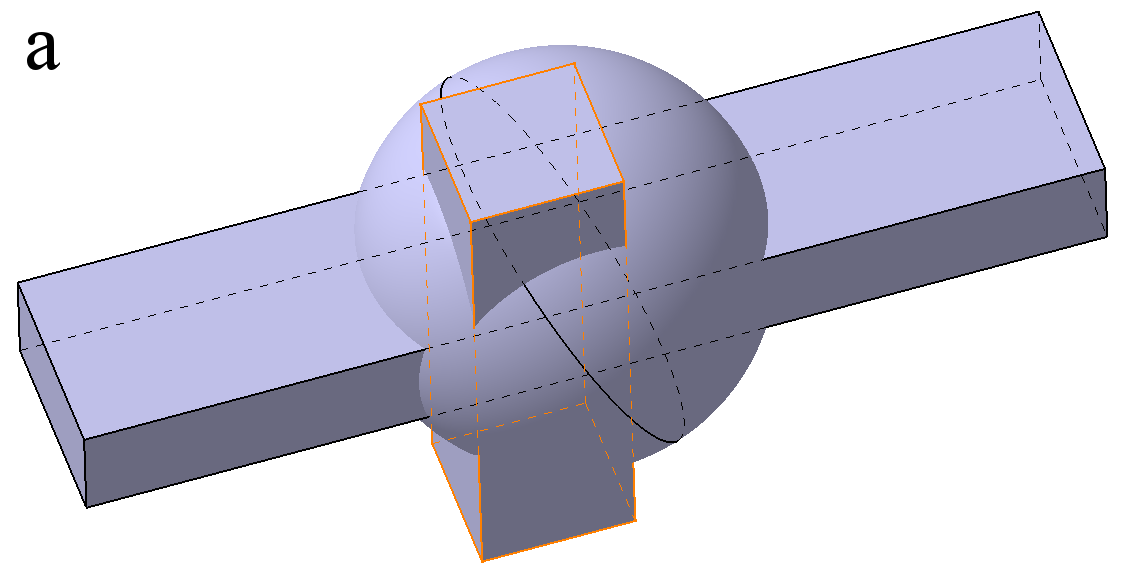
\includegraphics[width=1.0\textwidth]{pictures/DiffGeoRepr_a.png}
\end{minipage}
\hspace{0.01\textwidth}
\begin{minipage}[b]{0.495\textwidth}
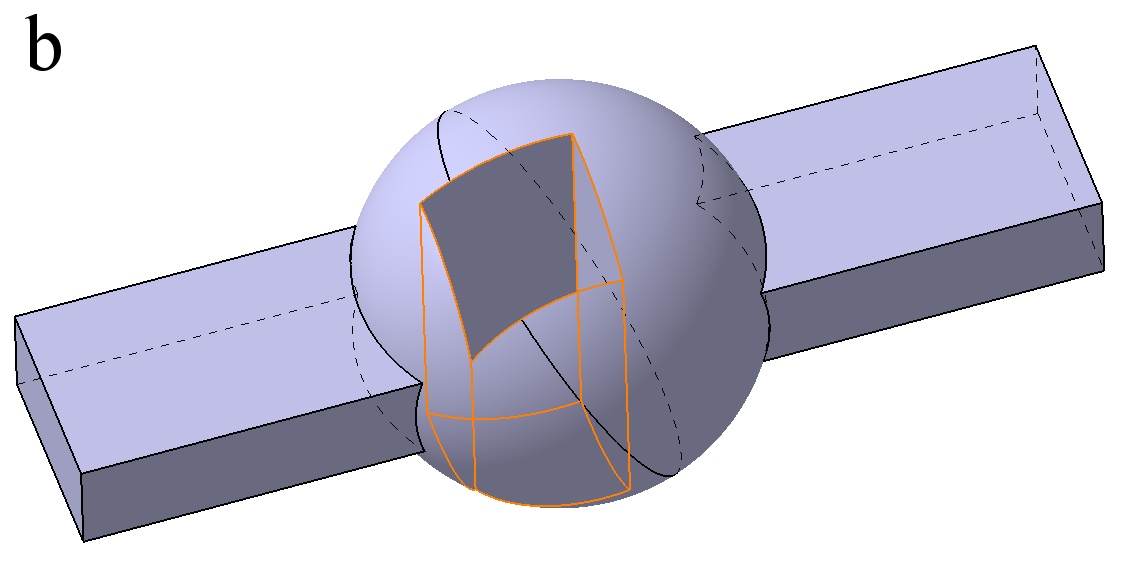
\includegraphics[width=1.0\textwidth]{pictures/DiffGeoRepr_b.png}
\end{minipage}
\begin{minipage}[b]{0.495\textwidth}
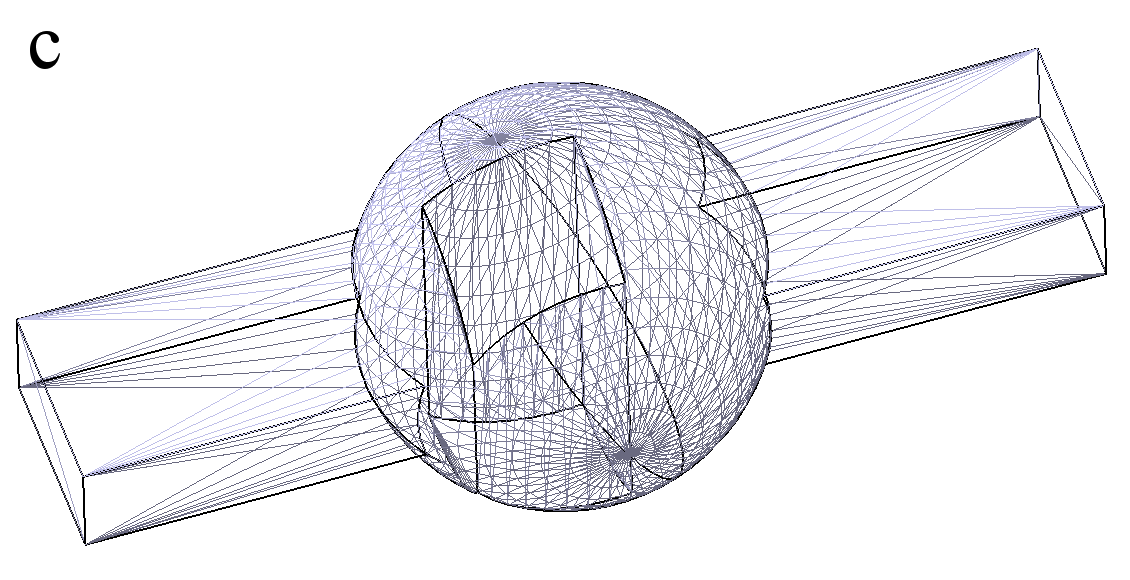
\includegraphics[width=1.0\textwidth]{pictures/DiffGeoRepr_c.png}
\end{minipage}
\hspace{0.01\textwidth}
\begin{minipage}[b]{0.495\textwidth}
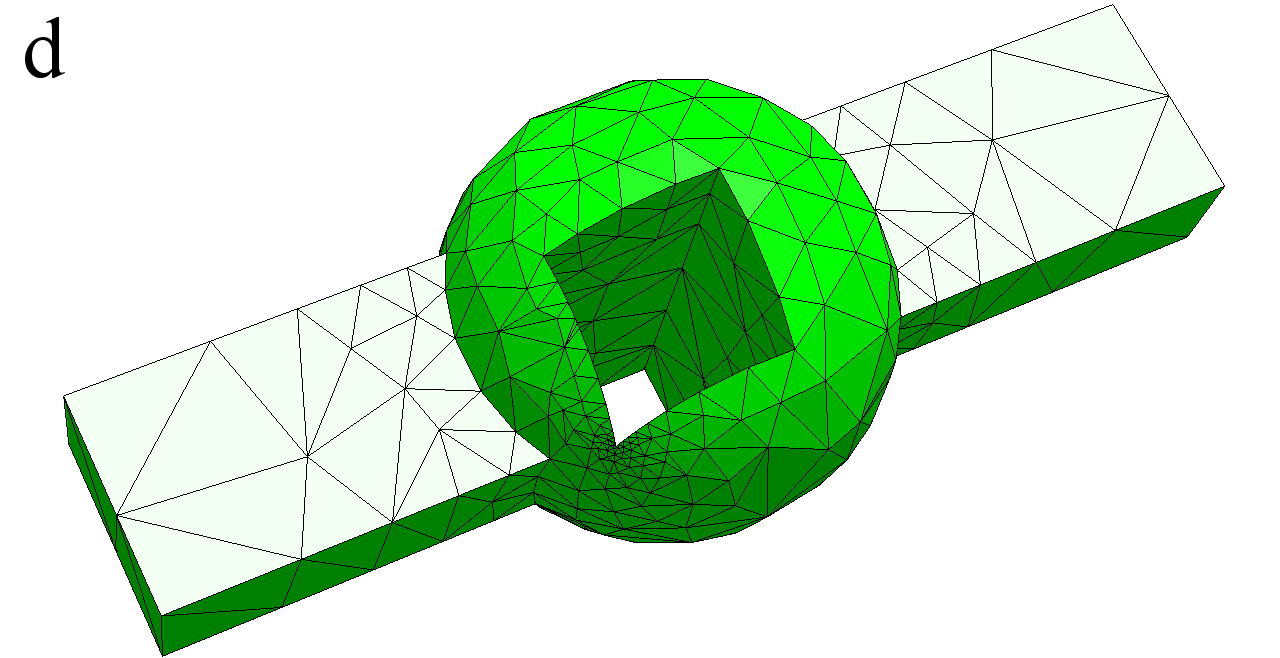
\includegraphics[width=1.0\textwidth]{pictures/DiffGeoRepr_d.png}
\end{minipage}
\caption{Одна и та же геометрическая форма, описанная различными представлениями: (a) отдельные примитивы до выполнения Булевой операции; (b) BREP после выполнения Булевой операции; (c) геометрия, триангулированная для визуализации; (d) КЭ-модель.}
\label{fig:DiffGeoRepr}
\end{figure}

% ================================================================================================================
%   ____                 __                            _       
%  / ___| ___  ___      / _| ___  _ __ _ __ ___   __ _| |_ ___ 
% | |  _ / _ \/ _ \    | |_ / _ \| '__| '_ ` _ \ / _` | __/ __|
% | |_| |  __/ (_) |   |  _| (_) | |  | | | | | | (_| | |_\__ \
%  \____|\___|\___/    |_|  \___/|_|  |_| |_| |_|\__,_|\__|___/
%                                                              
% ================================================================================================================

\subsection{Обмен геометрической информацией}\label{sec:secGeoFormats}

% \todo (например, BREP и триангулированная вместе в файле одного формата - ?)

Существует огромное множество форматов для обмена геометрией между различными программными продуктами. Следует различать геометрическое представление и формат, в котором данные записаны в файл. Существуют универсальные форматы, которые позволяют записывать в файл геометрию, представленную разными способами, но в большинстве случаев один формат подразумевает один способ представления геометрии. Данные могут быть записаны в файл как в виде текста, так и в бинарном виде. Проприетарные форматы в большинстве своём не имеют открытой спецификации, поэтому файлы этого формата бинарные, создаются и читаются ограниченным списком программ, в который, в первую очередь, входят продукты от фирм, являющихся авторами этих форматов. Также иногда эти фирмы дают возможность купить лицензию на модуль импорта/экспорта того или иного формата для реализации его поддержки в стороннем ПО.

Из множества популярных форматов для хранения и передачи геометрической информации, не подразумевающей перевод между различными представлениями, рассмотрим несколько наиболее употребимых в нашей области.

% \subsubsection{STEP}\label{sec:secSTEP}

\textbf{STEP} (STandard for Exchange of Product model data) --- независимый стандарт ISO-10303, получивший наибольшее распространение в инженерной практике для обмена информацией об изделии, в том числе геометрическими моделями.
%В наши дни практически любая САПР имеет возможность импорта и экспорта STEP.
%Данный стандарт предоставляет широкие возможности по обмену информацией об изделии.
Особенностью данного стандарта является наличие большого количества инструментов для описания BREP-геометрии. В то же время, следует отметить, что несмотря на то, что практические все современные САПР используют идентичные подходы к моделированию и имеют поддержку данного формата, STEP файлы не хранят дерево построения модели. По этой причине, даже если экспортировать STEP-файл из некоторой системы и импортировать обратно, то дерево построения, то есть последовательность формообразований, утеряется.
Обменные файлы STEP являются текстовыми. С одной стороны, это значительно упрощает разработку модулей для их импорта и экспорта, но с другой стороны, это приводит к тому, что для крупных моделей размер STEP-файлов становится достаточно большим, а следовательно и растёт время их обработки.

% \subsubsection{IGES}\label{sec:secIGES}

\textbf{IGES} (Initial Graphics Exchange Specification) --- независимый стандартизированный формат для обмена информацией между САПР, включая геометрические модели. В настоящее время многие САПР имеют поддержку IGES, однако данный формат можно рассматривать как устаревший, практически вытесненный стандартом STEP.

% \subsubsection{STL}\label{sec:secSTL}

\textbf{STL} (STereoLithography) --- текстовый формат для обмена тесселированной геометрией, который, возможно, является самым распространённым на данный момент форматом для передачи моделей в сфере 3d-сканирования и 3d-печати.

% \subsubsection{OBJ}\label{sec:secOBJ}

\textbf{OBJ} --- очень простой и открытый текстовый формат для обмена полигональными моделями. В файл OBJ записаны координаты вершин, списки индексов вершин каждого полигона и некоторые вспомогательные данные, типа текстурных координат и др.

% \subsubsection{CGR}\label{sec:secCGR}

% http://www.datakit.com/en/news/who-or-what-is-cgr--92.html

\textbf{CGR} (Catia Graphical Representation) --- проприетарный формат Dassault Systemes, используемый для хранения триангулированной модели, готовой для быстрой визуализации на дисплее. Позволяет одновременно, в одном файле, хранить несколько моделей, что широко применяется для хранения нескольких уровней детализации.
% \todo проверить

% \subsubsection{3DXML}\label{sec:sec3dXML}

%\textbf{3DXML} --- проприетарный формат Dassault Systemes, используемый для хранения триангулированной модели, готовой для быстрой визуализации на дисплее. 3DXML имеет закрытую спецификацию. Файл этого формата представляет собой архив с одним или несколькими геометрическими моделями и дополнительной информацией. 3DXML player --- это бесплатный продукт Dassault Systemes, позволяющий просматривать модели в файлах 3DXML.

% \subsubsection{VRML, WRL, X3D}\label{sec:secVRML}

%\textbf{VRML} (Virtual Reality Modeling Language). Файлы формата VRML имеют расширение wrl. \textbf{X3D} --- стандартизированный (ISO/IEC 19775/19776/19777) формат, являющийся наследником VRML.

% \subsubsection{COLLADA}\label{sec:secCOLLADA}

% https://www.iso.org/standard/59902.html
% https://en.wikipedia.org/wiki/COLLADA
% https://www.khronos.org/collada/

%Основанный на XML формат \textbf{COLLADA} (COLLAborative Design Activity) разработан специально для обмена геометрической информацией между интерактивными приложениями, такими как игровые движки, различные системы полигонального моделирования, САПР, и т.д. Файлы формата COLLADA имеют расширение dae (digital asset exchange). Формат COLLADA поддерживается некоммерческой организацией Khronos group, а в 2013 году был опубликован как международный стандарт ISO/PAS 17506:2012.

% \subsubsection{NEU, ANEU}\label{sec:secNEU}
% Простой текстовый формат для задания ...

% ================================================================================================================
%     _         _                                               _             
%    / \  _   _| |_ ___        ___ ___  _ ____   _____ _ __ ___(_) ___  _ __  
%   / _ \| | | | __/ _ \      / __/ _ \| '_ \ \ / / _ \ '__/ __| |/ _ \| '_ \ 
%  / ___ \ |_| | || (_) |    | (_| (_) | | | \ V /  __/ |  \__ \ | (_) | | | |
% /_/   \_\__,_|\__\___(_)    \___\___/|_| |_|\_/ \___|_|  |___/_|\___/|_| |_|
%                                                                             
% ================================================================================================================

\subsection{Возможности автоматического перевода между способами представления}\label{sec:secAutoConversion}

%Существует теоретическая возможность прямой конвертации из представления, принятого в GEANT/ROOT, в BREP, однако в процессе работы не было найдено существующей реализации подобного перехода. Конвертация в обратном направлении до настоящего времени не была математически описана, хотя теоретически также представляется возможной.

\begin{figure}[H]
\centering
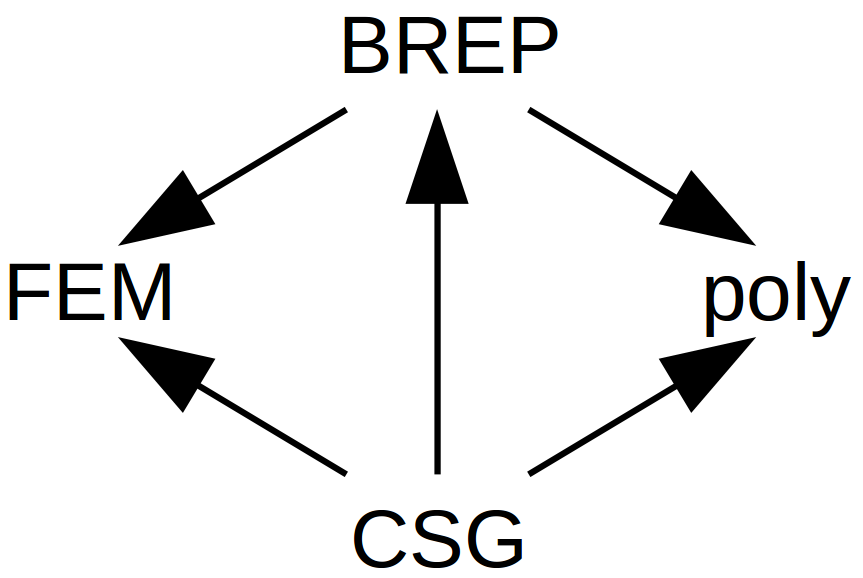
\includegraphics[width=0.3\textwidth]{pictures/Conversions.png}
\caption{}
\label{fig:Conversions}
\end{figure}

\subsubsection{Конвертация CSG в BREP}\label{sec:secCSGtoBREP}

Поверхности, используемые в качестве границ примитивов CSG --- это чаще всего поверхности, описываемые относительно простыми уравнениями; большая часть из них --- уравнения первого и второго порядка. Очевидно, что перевод отдельных примитивов в BREP-описание не представляет сложности независимо от вида уравнений, описывающих их границы --- для этого не требуется никаких дополнительных вычислений. Чуть более сложная задача, но всё же полность решённая, --- автоматический перевод формы, полученной в результате Булевой операции, в BREP-описание. В случае Булевой операции в CSG нет явного описания рёбер и вершин, полученных в результате пересечения отдельных граней примитивов, однако эти рёбра вершины напрямую получаются из параметров операндов и их позиционирования. Таким образом возможна быстрая и полностью автоматическая конвертация CSG-модели в BREP, и она реализована, возможно в неявном виде, во всех САПР.

Полная --- значит абсолютно все примитивы могут быть описаны с помощью BREP.

\subsubsection{Конвертация BREP в Polygonal}\label{sec:secBREPtoPolygonal}

Суть получения полигональной геометрии из полноценного BREP описания заключается в аппроксимации всех граней набором плоских фасеток. Очевидно, что если исходная грань не плоская, то аппроксиммирующая полиногальная сетка будет иметь от неё некоторое отклонение.
Давно разработаны и хорошо отлажены алгоритмы для такой аппроксимации. Точность аппроксимации --- управляющий параметр процедуры. Для более точной аппроксимации требуется больше полиногов, а следовательно возрастает нагрузка на графический адаптер.
% CSG -> poly
Из того что возможен автоматический перевод из CSG в BREP вытекает, что возможен также и перевод из CSG в полигональную.

Многие из них основаны на триангуляции Делоне, разработанной в начале 20~века.

Таким образом возможна полная и \todo беспроблемная \todo конвертация BREP-модели в полигональную, и она реализована, возможно в неявном виде, во всех САПР.

Полная --- значит абсолютно все примитивы BREP (точки, рёбра, грани) могут быть приблизительно, с заданной точностью, описаны полигональной сеткой. Управляющий параметр --- точность аппроксимации.

\subsubsection{Конвертация BREP в FEM}\label{sec:secBREPtoFEM}

Существуют алгоритмы, позволяющие эффективно получить разбиение исходной геометрической модели, например представленной с помощью BREP и построенной в САПР, на конечные элементы.
% CSG -> FEM
Из того что возможен автоматический перевод из CSG в BREP вытекает, что возможен также и перевод из CSG в КЭ-модель.

Первый этап процедуры разбиения твёрдого тела на конечные элементы заключается в триангуляции и выполняется теми же алгоритмами, что и для получения полиногальных моделей из BREP. Затем на основе разбиения граней строится пространственная сетка.
При этом инженер обычно глазами смотрит на сетку. Также при разбиении на сетку расчётчик руками даёт указания алгоритму. Например, на сколько элементов разбить то или иное ребро. Критерий построенной --- кривота элементов. Процедура разбиения тела на КЭ сложна и для более-менее сложной детали выполняется в несколько итераций. 

\subsubsection{Конвертация BREP в CSG}\label{sec:secBREPtoCSG}

Если тело (solid) представляет собой примитив, описанный средствами BREP (см. секцию~\ref{sec:geoCAD}), то представляется возможным реализовать алгоритм, распознающий этот факт и определяющий параметры примитива. Сначала необходимо выполнить проверку топологии тела (тело ограничено шестью плоскими гранями, стыкующимися по 12 рёбрам, и т.д.), затем выполнить геометрические проверки (перпендикурярность плоскостей, углы между рёбрами и т.д.). Задача усложнена тем, что за счёт богатых возможностей BREP фактически правильная фигура может быть описана бесконечным количеством способов. Можно привести следующий простой пример. Плоская прямоугольная грань может быть описана уравнением плоскости и замкнутым циклом из 4-х взаимноперпендикулярных рёбер (прямоугольник) на этой плоскости, а может быть разбита на два треугольника на той же плоскости, смежных по гипотенузе. Эти два описания обозначают геометрически эквивалентные формы, но во втором случае потребуется дополнительная процедура приведения двух треугольников к одному прямоугольнику --- суть, минимальному полному описанию.

Основной фактор, делающий невозможным полный перевод BREP-модели в CSG, заключается в том, что CSG имеет ограниченный список уравнений поверхностей, чаще всего не выше второго порядка, в то время как BREP позволяет задавать грани на основе поверхностей, описанных сложными уравнениями, например NURBS~\cite{NURBS}. Для описания таких сложных поверхностей можно прибегнуть к аппроксимации существующими в примитивах поверхностями. (\todo но это будет уже не полная конвертация)
Однако этот фактор является не главным, т.к. из практики известно, что подавляющее большинство геометрических форм в области детекторов --- достаточно простые.
Главная причина невозможности перевода из BREP в CSG заключается в том, что в подавляющем большинстве случаев форма тела не является примитивом. При переводе требуется каким-то образом представить её как результат Булевой операции.

% Описанные выше геометрические задачи также имеют следующую особенность. По причине ограниченности машинного слова числа с плавающей запятой хранятся в ПК с ограниченной точностью и выполнение расчётов, включающих матричные преобразования и тригонометрические функции, приводят к появлению заметных вычислительных ошибок. В большинстве случаев удаётся преодолеть эту проблему округлением до заданного знака, т.к. на практике в компьютерном геометрическом моделировании можно задаться физически обоснованным пределом снизу, например 1~мкм, или, с запасом, 1~нм, т.е. заведомо на много порядков выше точности вычислений. Но, к сожалению, это не всегда помогает.

% \subsubsection{Конвертация FEM в BREP}\label{sec:secFEMtoBREP}

% На практике не возникает необходимости переводить описание модели из КЭ в какое-либо другое. КЭ-модель всегда (кроме каких-то экстренных ситуаций) получена построением сетки на основе BREP или CSG. В КЭ-моделях границы тел описываются так же как и в полигональных. Следовательно, с теоретической точки зрения, перевод из FEM в BREP эквивалентен переводу из полигонального представления в BREP.

\subsubsection{Конвертация Polygonal в BREP}\label{sec:secPolyToBREP}

Если полиногами описана замкнутая оболочка, то представляется возможным объявить эту оболочку границой твёрдого тела, таким образом переведя без потерь полигональное описание в BREP, чтобы в дальнейшем работать средствами твердотельного моделирования. Если до цельности оболочки нехватает некоторого количества полигонов, то система обычно позволяет автоматически заполнить дыры плоскими фастеками, чтобы дальше можно было получить твёрдое тело.

% \todo Разобраться
Данная задача возникает при обработке результатов 3d-сканирования. 3d-сканеры выдают облако точек и первым этапом выполняется построение полиногальной модели по точкам. Затем обычно выполняется автоматизированное дополнение полинональной модели до замкнутой оболочки для получения твёрдого тела.

% Проблема имеет некоторое сходство с конвертацией CSG в BREP.

\textbf{Концентрируемся только на BREP, в котором описываются твёрдые тела, ограниченные замнутой оболочкой из поверхностей, либо большие непрерывные поверхности.}
